\documentclass{article}

% *****************************************************************
% Package things
% *****************************************************************
\usepackage[utf8]{inputenc}
\usepackage{mathtools}
\usepackage{amsmath}
\usepackage{amssymb}
\usepackage{enumitem}
\usepackage[hang,flushmargin]{footmisc}
\usepackage{booktabs}
\usepackage{color}
\usepackage{bbm}
\usepackage{footnote}
\usepackage{enumitem}
\usepackage{longtable}
\newcommand{\solution}[1]{{\color{blue}\fontfamily{cmss}\selectfont#1}}

\usepackage[anythingbreaks]{breakurl}

\usepackage{pgfplots}
\usepackage[margin=1in]{geometry}
\usepackage{hyperref}

\pgfplotsset{width=10cm,compat=1.9}


% *****************************************************************
% Estout related things
% *****************************************************************
\newcommand{\sym}[1]{\rlap{#1}}% Thanks to David Carlisle

\let\estinput=\input% define a new input command so that we can still flatten the document

\newcommand{\estwide}[3]{
		\vspace{.75ex}{
			\begin{tabular*}
			{\textwidth}{@{\hskip\tabcolsep\extracolsep\fill}l*{#2}{#3}}
			\toprule
			\estinput{#1}
			\bottomrule
			\addlinespace[.75ex]
			\end{tabular*}
			}
		}	

\newcommand{\estauto}[3]{
		\vspace{.75ex}{
			\begin{tabular}{l*{#2}{#3}}
			\toprule
			\estinput{#1}
			\bottomrule
			\addlinespace[.75ex]
			\end{tabular}
			}
		}

% Allow line breaks with \\ in specialcells
	\newcommand{\specialcell}[2][c]{%
	\begin{tabular}[#1]{@{}c@{}}#2\end{tabular}}

% *****************************************************************
% Custom subcaptions
% *****************************************************************
% Note/Source/Text after Tables
\newcommand{\figtext}[1]{
	\vspace{-1.9ex}
	\captionsetup{justification=justified,font=footnotesize}
	\caption*{\hspace{6pt}\hangindent=1.5em #1}
	}
\newcommand{\fignote}[1]{\figtext{\emph{Note:~}~#1}}

\newcommand{\figsource}[1]{\figtext{\emph{Source:~}~#1}}

% Add significance note with \starnote
\newcommand{\starnote}{\figtext{* p < 0.1, ** p < 0.05, *** p < 0.01. Standard errors in parentheses.}}

% *****************************************************************
% siunitx
% *****************************************************************
\usepackage{siunitx} % centering in tables
	\sisetup{
		detect-mode,
		tight-spacing		= true,
		group-digits		= false ,
		input-signs		= ,
		input-symbols		= ( ) [ ] - + *,
		input-open-uncertainty	= ,
		input-close-uncertainty	= ,
		table-align-text-post	= false
        }
% *****************************************************************
% Document starts here
% *****************************************************************

\begin{document}

\title{AK Replication a la Bayes}
\author{Rachel Anderson}

\maketitle

% Table 1
\begin{table}
\centering
\caption{OLS results using year/place of birth fixed effects and education dummies}
\estauto{ak_ols.tex}{1}{c}
\label{table1}
\end{table}

% Table 2
\begin{table}
\centering
\caption{IV resultst}
\estauto{iv.tex}{4}{c}
\label{table1}
\end{table}

%Table 3 -- will be first stage results 

\begin{figure}[h!]
\centering
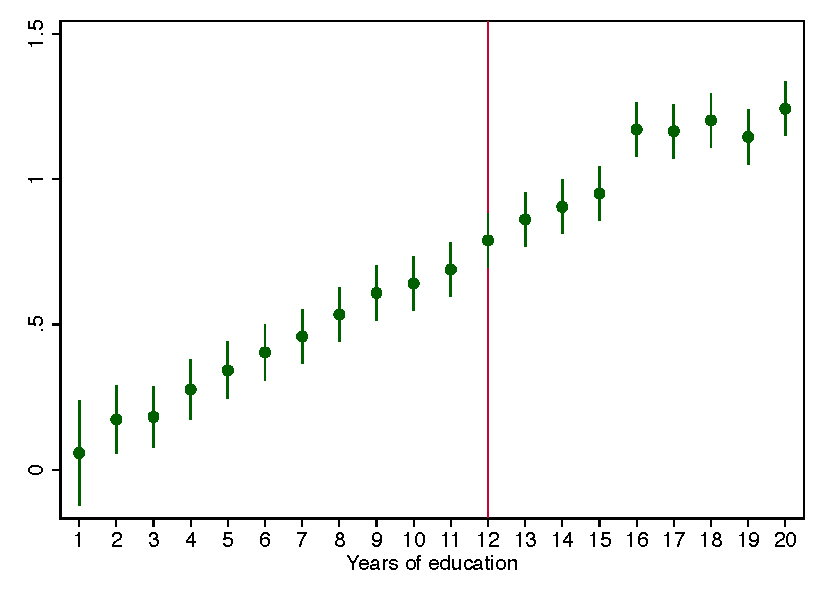
\includegraphics[width=0.7\textwidth]{../Figures/coefplot_ols.pdf}
\caption{Plot of OLS coefficients for education variables}
\end{figure}

\begin{figure}
\centering
  \begin{minipage}[b]{0.48\textwidth}
    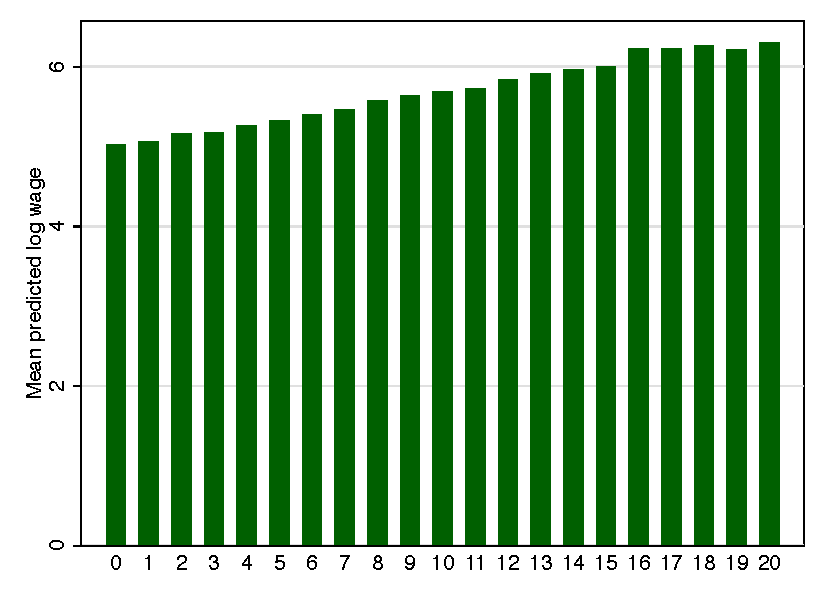
\includegraphics[width=\textwidth]{../Figures/logwage_ols.pdf}
    \caption{Predicted log-wage by education level}
    \label{fig:1}
  \end{minipage}
  \begin{minipage}[b]{0.48\textwidth}
    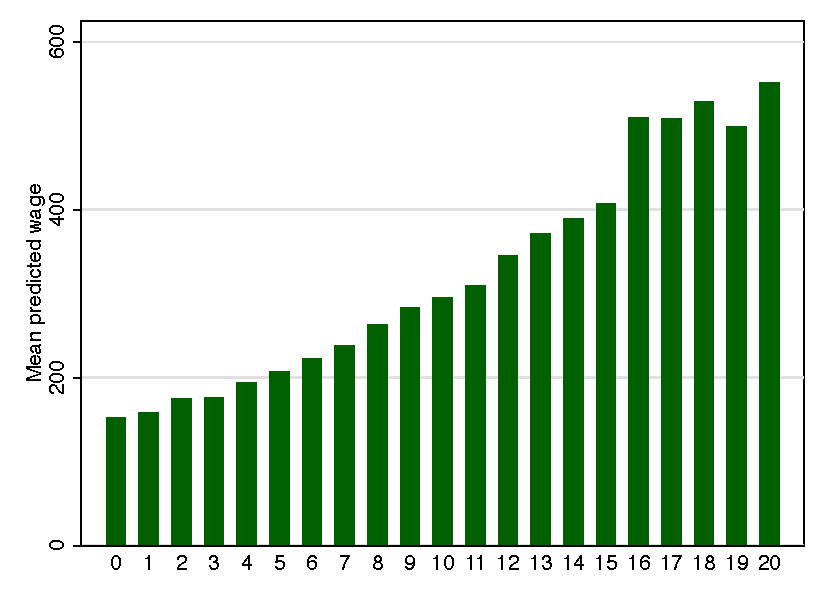
\includegraphics[width=\textwidth]{../Figures/wage_ols.pdf}
    \caption{Predicted wage by education level}
    \label{fig:2}
  \end{minipage}
\end{figure}

\end{document}